%% go to the website http://en.wikibooks.org/wiki/LaTeX For Help 
\documentclass[11.5pt]{article}
%Math Related Packages
\usepackage{mathtools}
\usepackage{amsmath}
\usepackage{amsfonts}
\usepackage{amssymb}
\usepackage{relsize}
% Pseudocode Packages
%\usepackage{algorithm}
%\usepackage{algpseudocode}
\usepackage[colorinlistoftodos]{todonotes}
% Automata/Graph Packages
\usepackage{tikz}
\usepackage{pgf}
\usetikzlibrary{arrows,automata}
\usepackage[latin1]{inputenc}
\usetikzlibrary{automata,positioning}
%%%Formatting Options for Pages
%\usepackage[a4paper,left=2cm,right=2cm]{geometry} %Change Margins
\usepackage[colorlinks=true, allcolors=blue]{hyperref} % adds hyperlinks
\usepackage{listings}
\usepackage{multicol}
\usepackage{perpage}
\MakePerPage{footnote}
%%%Graphics Packages and Caption Tools
\usepackage{graphicx}
\usepackage{fullpage}
\newcounter{Figure} 
\setcounter{Figure}{1}
%\usepackage{slashbox}
\usepackage{ulem}
\usepackage{csvsimple}
%%%Colors Package with Custom Defined Colors
\usepackage{color}
\usepackage{colortbl}
\definecolor{codegreen}{rgb}{0,0.6,.2}
\definecolor{codegray}{rgb}{0.5,0.5,0.5}
\definecolor{codepurple}{rgb}{0.58,0,0.82}
%%Custom Functions and Commands
\newcommand\indentFour{\indent\indent\indent\indent}
\newcommand\indentThree{\indent\indent\indent}
\newcommand\indentTwo{\indent\indent}
\newcommand\tab{\ \ \ }
\newcommand\proof{\setcounter{equation}{0}\hfill\fbox{\rule{.02in}{0pt}\rule[0ex]{0pt}{.5ex}}}

%%Math Commands
\newcommand{\Lbra}{\left\langle}
\newcommand{\Rbra}{\right|}
\newcommand{\Rket}{\right\rangle}
\newcommand{\Lket}{\left|}
\newcommand{\bra}[1]{\Lbra #1 \Rbra}
\newcommand{\ket}[1]{\Lket #1 \Rket}
\newcommand{\braket}[1]{\Lbra #1 \Rket}
\newcommand{\Exists}{\ \exists \ }
\newcommand{\Forall}{\ \forall \ }
\newcommand{\abs}[1]{\left| #1 \right|}
\newcommand{\Frac}[2]{\left(\frac{#1}{#2}\right)}
\newcommand{\Mat}[1]{\left[\begin{matrix} #1 \end{matrix}\right]}
\newcommand{\vhi}{\varphi}
\newcommand{\R}{\ \mathbb{R}}
\newcommand{\C}{\ \mathbb{C}}
\newcommand{\N}{\ \mathbb{N}}
\newcommand{\Z}{\ \mathbb{Z}}
\newcommand{\I}{\ \mathbb{R/Q}}
\newcommand{\x}{\mathrm{x}}
\newcommand{\mbf}[1]{\mathbf{#1}}
\newcommand{\Dpart}[2]{\frac{\partial #1}{\partial #2}}
\DeclarePairedDelimiter{\ceil}{\lceil}{\rceil}
\newcommand{\U}{\underline}
%Numbering
\newcounter{graphics}
\newcounter{tables}
\renewcommand{\abstractname}{Abstract}

\begin{document}
\title{Deep Learning for Knowledge Graph Completion}
\author{Nick, Kevin, Cesar Bartolo-Perez, Doug\\
	{\small\textit{University of California - Davis}}
} 
\date{November 30th, 2017}
\maketitle
\rule{\textwidth}{1pt}



\begin{abstract}

\end{abstract}

\tableofcontents


\section{Introduction}



\section{Methods}
\subsection*{Multilayer Perceptron Model (MLP)}


\paragraph{} The dataset we considered was queried from the WikiData, a free opensource knowledge base that acts as the central storage device for its sister projects including Wikipedia, Wikivoyage, and Wikisource \cite{Wikidata}. Wikidata offers a SPARQL type queries for obtaining data on a variety of sources. We queried data regarding the lineage of many famous people in history including: Frederik, Crown Prince of Denmark, George Windsor, Earl of St Andrews, and Shigeko Higashikuni. The relations we considered were if one person, or entity, was the Father, Mother, Spouse, Sibling, or Child of another. See Figure \ref{query} for an example of the query we used to obtain our dataset. 


\begin{figure}[h!]
 \lstinputlisting[language=Matlab]{code/SparqlQuery.txt}
 \caption{SPARQL query used to obtain our raw data from Wikidata}
 \label{query}
\end{figure}


\paragraph{} The raw data is a table of values that lists each person and their Father, Mother, spouse, sibling, and child; leaving an entry empty if unknown. We processed this table into positive triplets of the form \texttt{(Q193752, P25, Q229279, 1)} where \texttt{Q193752} and \texttt{Q229279} are a unique encoding of the target and related entities respectively, \texttt{P25} represents one of the relations, or predictes, and \texttt{1} indicates that this statement is true. In english this triplet implies that \texttt{Q229279} is the \texttt{P25} of \texttt{Q193752}. These positive facts represent all the data we can pull directly from the knowledge graphs. However, to increase the robustness of our data, we can create negative facts as well. For example, since we know that Cleopatra VII Philopator, the last active pharaoh of Ptolemaic Egypt, was the daughter of Ptolemy XII Auletes, we can conclude she was not the daughter of Richard Nixon. Thus we can extend our data to contain these negative triplets of the form \texttt{(Q1,P1,Q2,-1)}. In all, we were able to produce 37395 positive triplets and 37391 negative triplets from our raw data. 

\paragraph{} In an effor to exploit the uniqueness in the names for each of our entities, we used word embeddings of each of the words in a name to generate entity embeddings. We used the Fasttext model to generate word embeddings from semantic anaylsis across Wikipedia. Fasttext is a library that represents words as bags of character $n$-grams for fast and efficient classification \cite{BojanowskiGJM16,JoulinGBM16}. Thus, we used Fasttext to obtain $300\times 1$ word embeddings of each of the unique words found in all of our entitie's names. For example, the name "Charles Stuart, 1st Earl of Lennox", we found an 300 dimensional embedding vector for Charles, Stuart, 1st, Earl, of, Lennox. Once each of the words had embeddings, we could construct entity embeddings for each of our entities. The method we used for this was to aggregate the word embeddings by taking the mean across each of the words within an entity name. For the MLP model, if Fasttext could not produce a valid embedding for a given word, then that word was ignored. Moreover, if an entity consisted entirely of unknown words, then that entity was thrown out. We did this to preserve the integrity of our input data because in the standard MLP model we would not be training these embeddings. However, for more complex models, another suitable technique is to randomize the embeddings for these entities, or all entities, to guarantee a more representative dataset. Overall, only about 6.4\% of the entities had no suitable embedding. Once we encoded each entity with their embedding we produced a dataset where each row contains the numeric representation of a triplet. Hence, for a triplet given by \texttt{(EntityA,Pred2,EntityB,1)}, where the embedding for \texttt{EntityA} and \texttt{EntityB }is $[a_1,a_2,\cdots,a_{300}]^T$ and $[b_1,b_2,\cdots,b_{300}]^T$ respectively, the associated row in our data set is given by
$$ \Mat{a_1,a_2,a_3,\cdots,a_{300},b_1,b_2,\cdots,b_{300},0,1,0,0,0} $$
where the last 5 columns represents the truth values for each of the 5 predicates (Father, Mother, Spouse, Sibling, Child).

\paragraph{} One we had a comprehensive dataset to train on, we designed our predictive model. We implimented a Multiyaler Perceptron (MLP) model using the RSNNS package following the Stuttgart Neural Network Simulator\cite{RSNNS}. Figure \ref{MLPArch} shows a general look at the architecture for our MLP design. We tested a few variations of the MLP model to determine the suitable parameters for our dataset; including a variable number of layers, activation functions, and nodes per layer. Moreover, we tuned the hyperparameters such as the learning rate and momentum term for backpropagation. We will reference Figure \ref{MLPArch} as we discuss the effects of the different architectures. 


\begin{figure}[h!]
 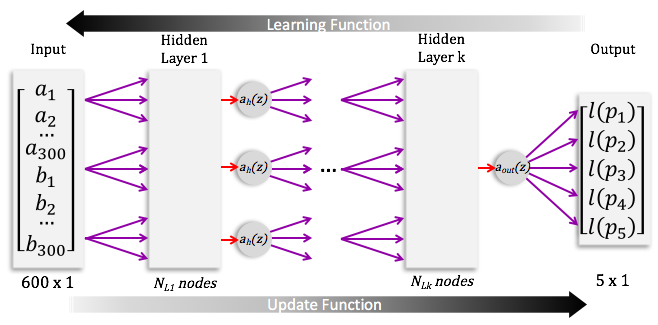
\includegraphics[width=1\textwidth]{report_mlp/GenArchitecture.png}
  \caption{A general look at the Neural Network architecture used for a MLP model with $k$ hidden layers with $N_{L_i}$ nodes for the $i$th layer, a common activation function $a_h(z)$ for each layer, and a final output activation function $a_{out}(z)$. We have 600 features from our input, 1 for each dimension of both entity embeddings, and we are predicting the true/false value of our 5 output predicates. Note that $l(p_1)$ is the likelihood that the predicate $p_1$ is true.  }
  \label{MLPArch}
\end{figure}


Where we have used standard backpropagation and backpropagation with momentum methods in our simulation models.

Different  MLP architectures are built, varying number of hidden layers, nodes and iterations in order to improve the accuracy and precision of our model.

Weighted SSE by number of iterations of the training and tetsing sets in addition to ROC curves will provide the references in our model architecture selection.

\section{Results}

In order to prevent overfitting in our model, we have compared our model with 100 and 50 interations (Figure \ref{50_100_128.png}). We can notice that under 100 iterations, the trainin error drops to a weigthed SSE of almost 500. However, our testing error, start increasing after 30 itearions aproximately. From this results, we can infer that we have reached an overfitting in our model and a smaller number of iterations are enougth. In that sense, we have run our model with 50 iterations, avoiding the increase in the SSE.\par
 

\begin{figure}[h!]
 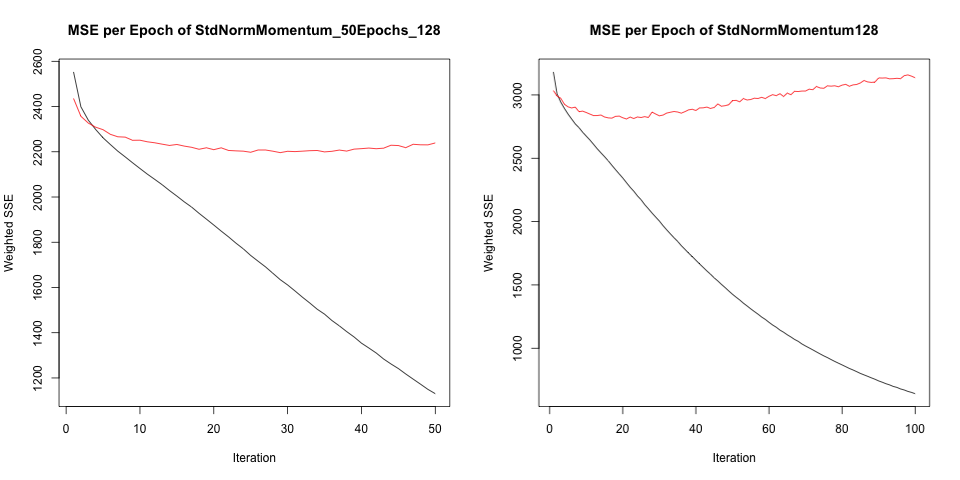
\includegraphics[width=1\textwidth]{report_mlp/50_100_128.png}
  \caption{MSE at different iterations. The structure presents a single hidden layer with 128 nodes}
  \label{50_100_128.png}
\end{figure}


In a second running of the model, we have added a new hidden layer  with different number of nodes (16,64 and 128). Before 50 iterations, adding nodes to the second hidden layer, reduce the error in our model. However, after 50 iteration, the higher number of nodes, increase rapidly the overfitting  of the model. \par 


\begin{figure}[h!]
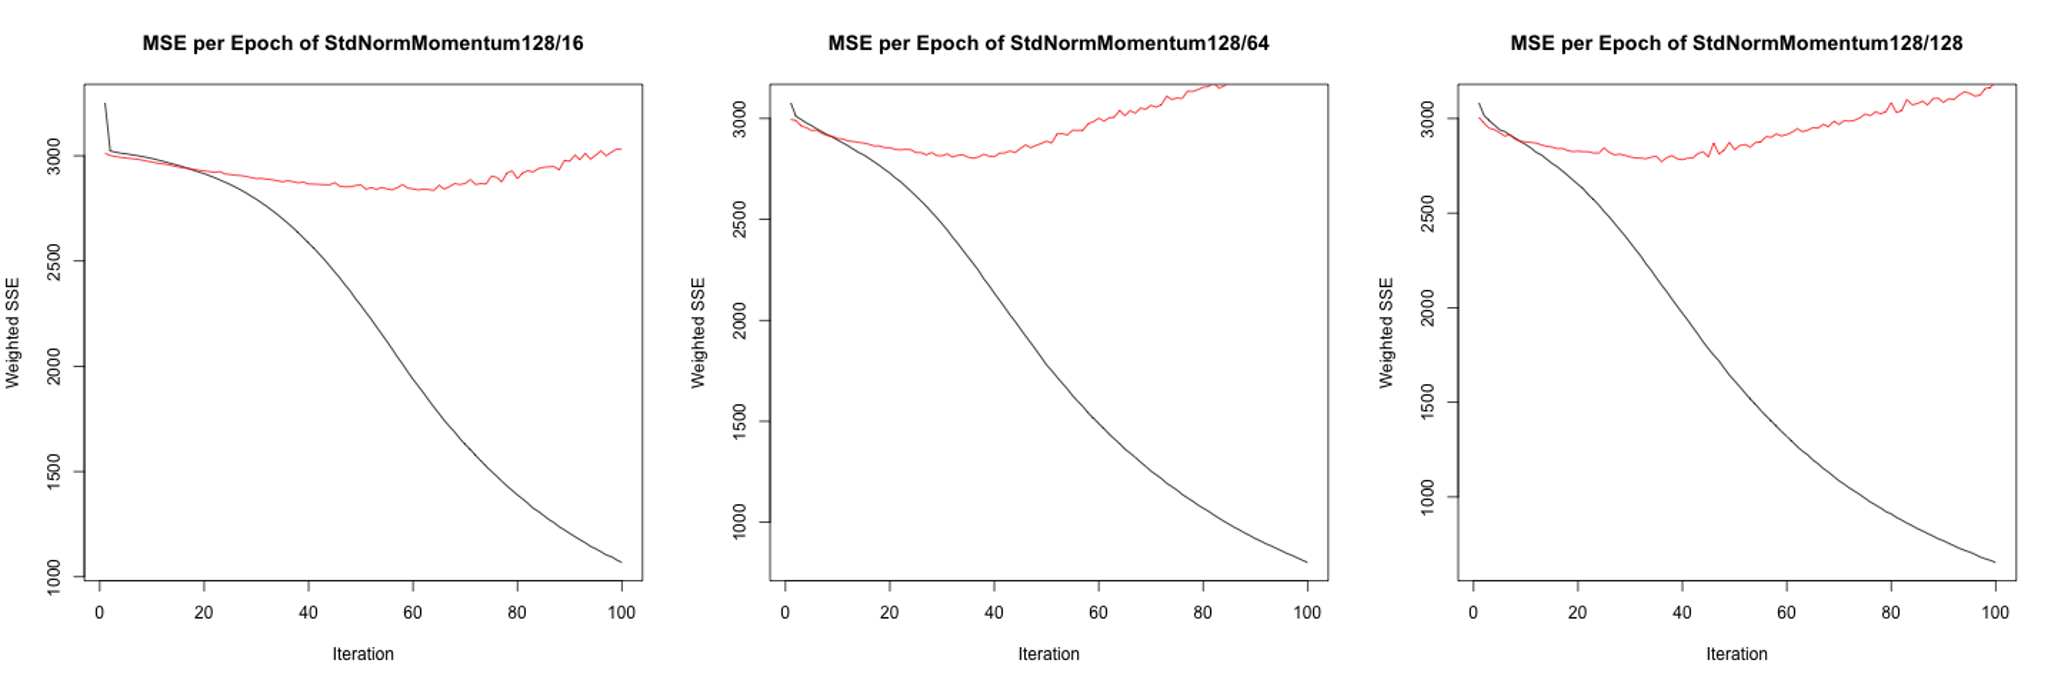
\includegraphics[width=1\textwidth]{report_mlp/128-16_64_128.png}
  \caption{MSE for A NN with two hidden layers with different nodes at second hidden layer.}
\label{128-16_64_128.png}
\end{figure}

In  a following set of tests, we compared different Neural Networks structures, increasing the number of hidden layers (hidden layers/nodes: 128, 128/16 and 128/128/16).  Figure \ref{128-16_64_128.png} shows that for the model with three hidden layers the training error is not decreasing considerably before 40 iteration. Suddently, the SSE in this NN structure drops abruptaly. The training error, shows that the error keep increasing at that range of iterations. This beahvior, can be attributed to an overfitting in our model. \par

Ths trend described above is similar for two hidden layers. For teh case of just one hidden layer with 128 nodes, the error does not drop abruptaly for the training set but we can see an increase in the error for after 30 iterations aproximately. \par 

These results, make us suggest that only one hidden layer is enough for our MLP model, since there is not a big improvement in the reduction of error with more layers added and with the benefit of less computational resources are required.
This decision is confirmed comparing their ROC curves for each NN structure.
 








\begin{figure}[h!]
  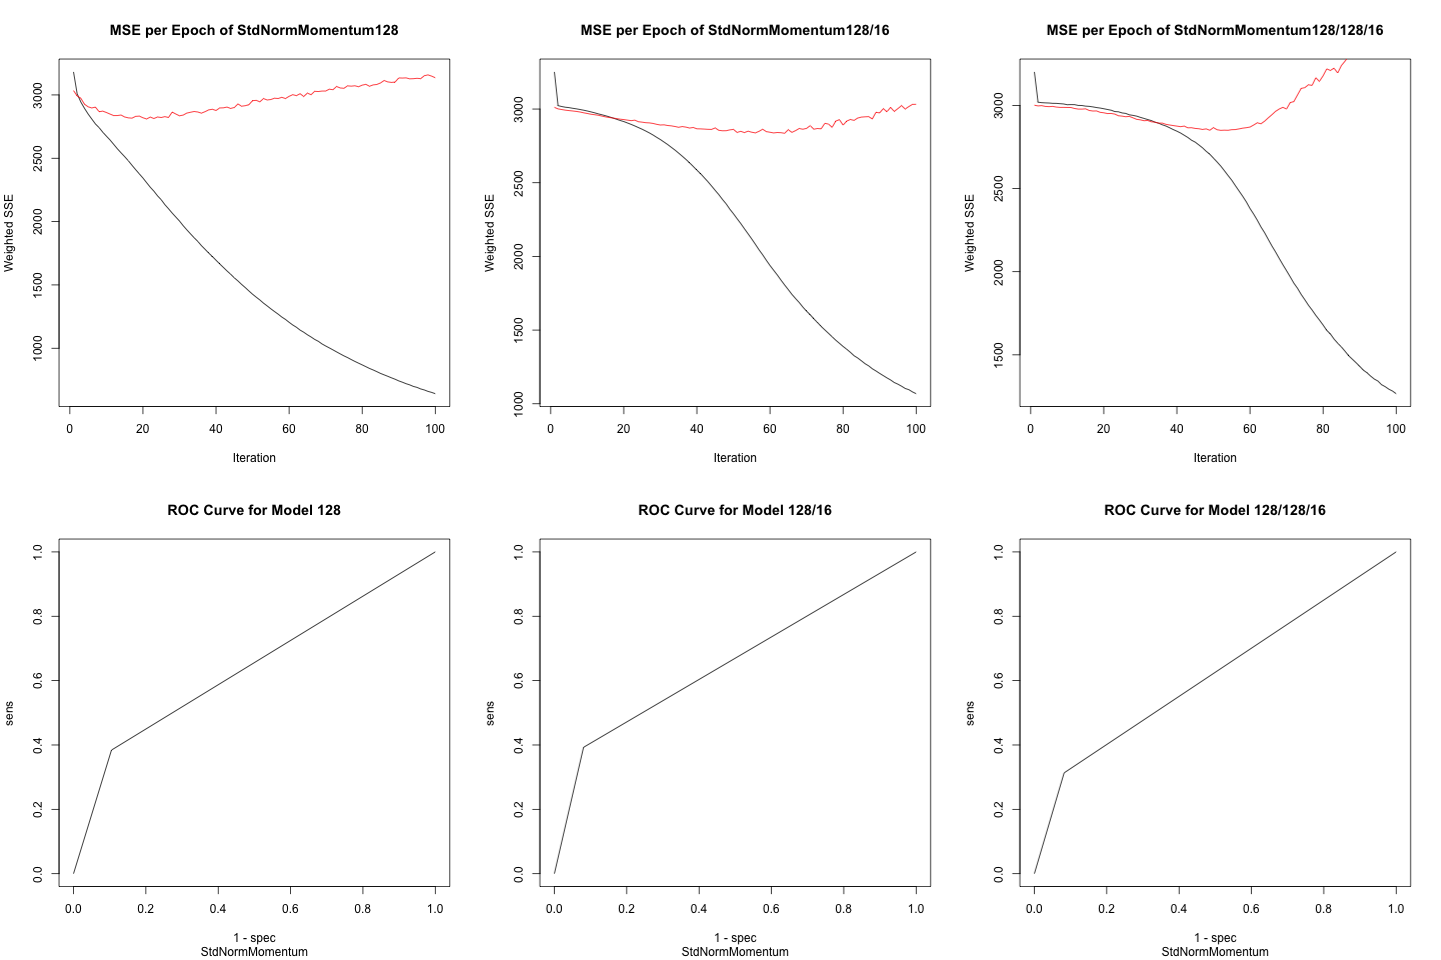
\includegraphics[width=1\textwidth]{report_mlp/different_layers_MSE_ROC.png}
    \caption{MSE and ROC curves for different levels of hidden layers}
    \label{different_layers_MSE_ROC.png}
\end{figure}



\section{Discussion}

\bibliographystyle{ieeetr}
\bibliography{bib}{}

\end{document}